\documentclass[12pt, a4, epsf] {article}
%==================================================
%Mypackages
\usepackage{epsf, amsmath, amssymb, graphicx, epsfig, amsthm}

\usepackage{subfigure} % For subfigures
\usepackage{setspace} 
\usepackage{fancyhdr} 
\usepackage{eurosym}  %To write a Euro symbol
\usepackage[euler]{textgreek}
\usepackage[english]{babel}
\usepackage[utf8]{inputenc}
\usepackage[colorlinks = true, urlcolor = blue, linkcolor = blue]{hyperref}
\usepackage{graphicx}
\usepackage{float}
\usepackage{bbm}
\usepackage{placeins}
\usepackage{pdfpages}
\usepackage{listings}
\usepackage{tikz}
\usetikzlibrary{graphs,graphs.standard}
\usetikzlibrary{shapes.geometric}
\usetikzlibrary{trees}
\usepackage{forest}
\usepackage{pdfpages}
\usepackage{algorithm} 
\usepackage{algpseudocode} 
%\usepackage[round]{natbib}


%Could change text height, width etc. 
\oddsidemargin 0mm
\evensidemargin 0mm
\textheight=24cm
\textwidth = 16cm
\topmargin= -1cm 

%Definition for theorems, definitions etc. for English texts
\theoremstyle{plain}
\newtheorem{theorem}{Theorem}[section]
\newtheorem{definition}[theorem]{Definition}
\theoremstyle{definition}
\newtheorem{example}[theorem]{Example}
\newtheorem{remark}[theorem]{Remark}


%==================================================
%My commands: Define your commands here:

\begin{document}
\begin{center}

{\Large Dummy Title\\}
By Dummies \\
27 JUN 2020
\end{center}

\section*{Abstract}
Public transportation plays a vital role connecting people with each other. International trade and tourism is reliant on commercial aviation. And the most successful cities all have buses, trams, or subways connecting workers to their workplaces. However, the speed and connectivity of these transportation networks leave us vulnerable to disease propagation.\\

In this paper, we introduce a general agent-based framework for modeling disease spread on transportation networks. We use it to build models of major transportation networks, and take a special look at the New York City subway to see how well it can predict infection rate and infection hotspots during the 2020 COVID-19 epidemic.\\

We found that countermeasures significantly impacted the spread of coronavirus and that there is a correlation between infection hotspots and subway lines as well as commute time.

\section*{Competencies Briefing (for other NS teams)}
\textbf{Purpose: Brief others on competencies so we can discuss things\\}
\textbf{Transportation Networks\\}
\textit{specifically NYC subway, world airline network, Madrid trains, Moscow metro. mapping, passenger flow\\}
\textbf{python, networkx, mesa\\}
\textit{we're working with these techs.\\}
\textit{Writer's Note: Obviously to be removed before submission\\}
\textit{This report was last pushed to OverLeaf on 20.06.2020. You will find our latest work at the link below:}
\url{https://github.com/cheung-ho-lum/NS_Epidemics_ABM_Approach/blob/master/Report/ABM_NYC_Subway.pdf}

\section*{Background}
\subsection*{Epidemics and COVID-19}
Coronavirus disease 2019 (COVID-19) is a disease caused by the SARS-CoV-2 coronavirus. Since being identified in December 2019, it has been labelled by the WHO as a pandemic, and spread around the world. Epidemics such as the 'coronavirus' have been a subject of research for centuries, and is of special interest to those working in public health. Recent waves of new research came in 2002 (SARS), 2009 (H1N1), and 2014 (Ebola). However, in these prior epidemics, researchers did not have access to as much data as we have currently. In recent years, the state of data science research tools have also greatly improved, allowing researchers to answer questions in novel ways, but following the scientific method. In this paper, we will try to respect the expertise of public health researchers, medical professionals, and the general public by being conservative when making conclusions.

\subsection*{COVID-19 in NYC}
In addition to general background knowledge about COVID-19, it would behoove the reader to know about the early spread of the disease in New York. Analysis of viral RNA in patients at the Mount Sinai Health System[\textbf{citation}] has lead researchers to conclude that the virus first came into the community through "multiple, independent but isolated introductions" from Europe and elsewhere in the USA. Below we have also given an approximate timeline of some of the most relevant events as of June 1st, 2020. We would also like to note that as forensic researchers begin examining the data, some significant new dates or corrections may arise:\\ 
\begin{itemize}
	\item February 25 - First positive test in NYC from a 39 year-old female healthcare worker flying back from Iran.
	\item March 3 - First confirmed P2P spread in NYC.
	\item March 9 - Mayor holds press conference and notes that there have been 16 confirmed cases.
	\item March 12 - Mayor declares a local state of emergency.
	\item March 15 - Schools officially close.
	\item March 22 - State order (PAUSE) to shelter in place comes into effect.
\end{itemize}
\subsection*{COVID-19 and the NYC Subway}
On April 24th, 2020, a researcher at MIT released a working paper finding that "The Subways Seeded the Massive Coronavirus Epidemic in New York City"[\textbf{citation needed}]. The paper received a lot of attention from the media. There is, at least, significant correlation between subway lines and severity of infection. But the factors involved are unknown and disputed. For example, high infection rate could be rated to dense housing, and housing is denser around subway stations[\textbf{citation needed}]. 

From this paper, and other prior research into subways, we bring into our own work two major points about disease spread on subways:\\
\begin{itemize}
	\item Infection on a subway network depends much more strongly on the line than the geographical distance or network shortest path between stations.
	\item Infection on a subway network depends on the average commute time of commuters using the station.
\end{itemize}

An another important piece of information is the subway ridership. The NYC Metropolitan Transit Authority (MTA) publicly releases turnstile data. Below we show a figure demonstrating the gradual shutdown of NYC between March 9th and March 23rd.
\begin{figure}
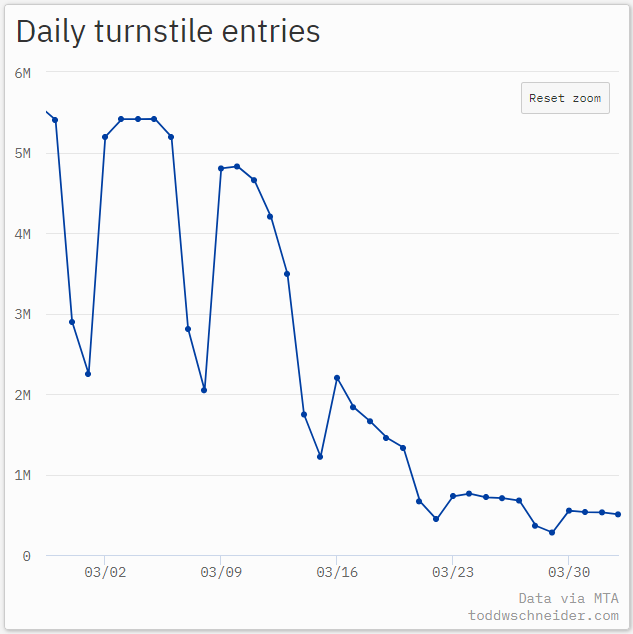
\includegraphics[width = 1.0\textwidth]{Scratch_Visuals/schneider_ridership.png}
\end{figure}

\subsection*{Epidemic Modeling}
There are two basic types of modeling for epidemics. Statistical and Mechanistic. While statistical modeling has typically given more accurate forecasts for a well-known situation [citation needed], mechanistic models such as the SIR and SEIR compartmental models help to explain why phenomena such as epidemics spread the way they do, and what impact various policy decisions will have on the result.
\subsection*{SEIR Model}
As we will be using the SEIR model in our research, we will cover it briefly here. The SEIR compartmental model is a mathematical modeling of infectious diseases where a closed population of people move successively from compartments suspected to exposed to infected and to removed. We briefly provide an explanation of each compartment and leave the equations below.
\begin{itemize}
	\item \textbf{Susceptible} - These people are susceptible to getting the disease from someone infected.
	\item \textbf{Exposed} - These people are no longer susceptible to the disease, and do not infect others. After a latent period, they become infectious.
	\item \textbf{Infected} - These people will spread the disease to susceptible people. After a period of time they are removed by recovery, hospitalization, death.
	\item \textbf{Removed} - Sometimes known as resistant or recovered. We will do our modeling with the term 'removed'. These people are no longer spreading the disease.
\end{itemize}
\textit{Writer's note: just take the equations from someone's overleaf}
\begin{align*}
dS/dt \\
ds/dt = - beta * s(t) * i(t) \\
de/dt = beta * s(t) * i(t) - alpha * e(t) \\
di/dt = alpha * e(t) - gamma * i(t) \\
dr/dt = gamma * i(t) \\
S + E + I + R = 1 \\
\end{align*}
\subsection*{Newer Compartmental Models}
While we have done some research into more advanced models and are interested in cases such as super-spreaders, we believe the SEIR model to be sufficient for the modeling done in this paper. Basic SIR is insufficient because public health officials often make policy decisions based on positive case numbers. For example, an official may decide to impose strict isolation only after 100 positive cases. But by the time there are 100 cases of 'infected' people, there may be 1000 exposed people who will meaningfully impact epidemic statistics.
\subsection*{Epidemics on Transportation Networks}
\textit{Writer's Note: epidemics on social networks blah blah linear threshold}
\textit{epidemics on transportation networks a little different, passenger flow is one of the most important numbers}
\subsection*{Agent Based Models}
It's just a tool. like any model. Simulating agents in an environment. Key parameters are agent, model, and environment parameters. For example, we have the following list thus far:\\
\begin{verbatim}
	(Agent)STATUS_SUSCEPTIBLE = 'Susceptible'
	(Agent)STATUS_EXPOSED = 'Exposed'
	(Agent)STATUS_INFECTED = 'Infected'
	(Agent)STATUS_INFECTED_ASYMPTOMATIC = 'Asymptomatic'
	(Agent)STATUS_RECOVERED = 'Recovered'
	(Agent)TIME_TO_RECOVER = 10
	(Agent)TIME_TO_INFECTION = 3
	(Model)RUN_SPAN = 60
	(Model)TOTAL_POPULATION = 50000
\end{verbatim}
The environment is new york subway mapped as a network.\\ 
All of this is still being discussed.\\
\subsection*{Transportation Networks and Epidemics}
\subsection*{Airlines}
\subsection*{Subways and Subway Nomenclature}
This guy is indispensable for figuring out how to parse some of this data:\\
\url{https://en.wikipedia.org/wiki/New_York_City_Subway_nomenclature}\\
\textbf{The key is lines and routes}\\
\section*{Methodology}
\subsection*{MESA(Or our ABM)}
\textit{Writer's note: I'm a bit too lazy to learn tikz-uml. I'll just make a regular uml and... screenshot it\\}
\begin{figure}
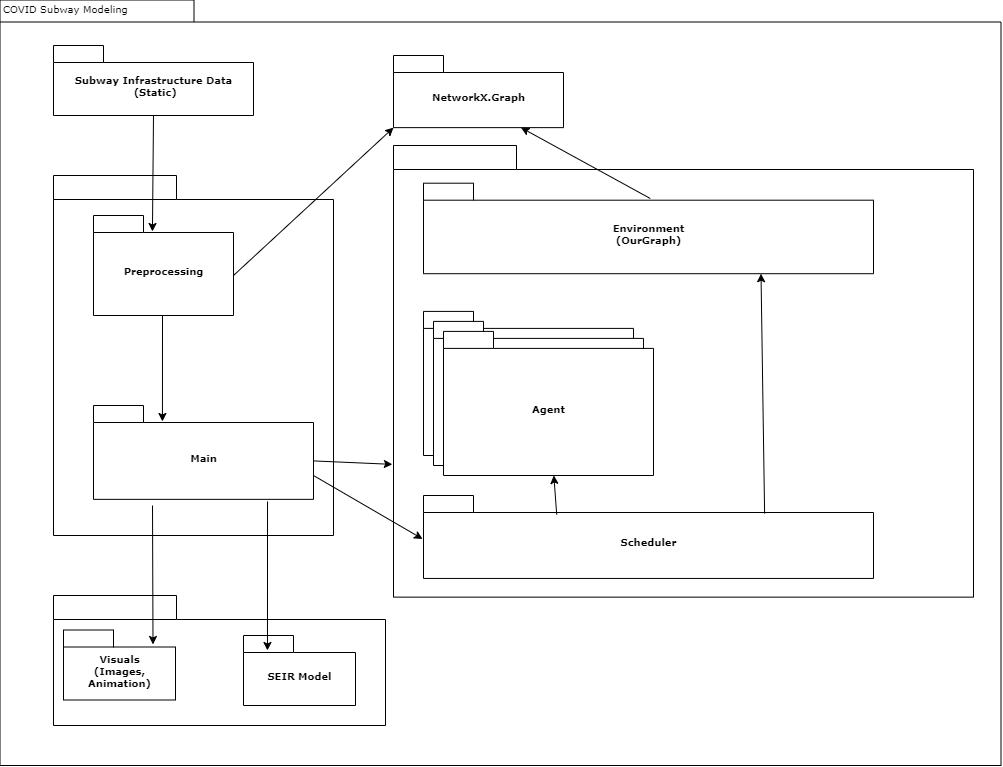
\includegraphics[width = 1.0\textwidth]{Scratch_Visuals/covid_subway.png}
\end{figure}
\subsection*{NetworkX}
\subsection*{MTA Station Data}
\textbf{Station, Complex, Line, Route\\}
\textit{station 167... doubled\\}
\textit{making edges. GTFS Data... no we do it ourselves\\}
\subsection*{MTA Turnstile Data}
\textit{discuss format. every 4 hours, every machine. aggregation.\\}
\section*{Fitting the data}
\FloatBarrier
\begin{figure}[htbp]
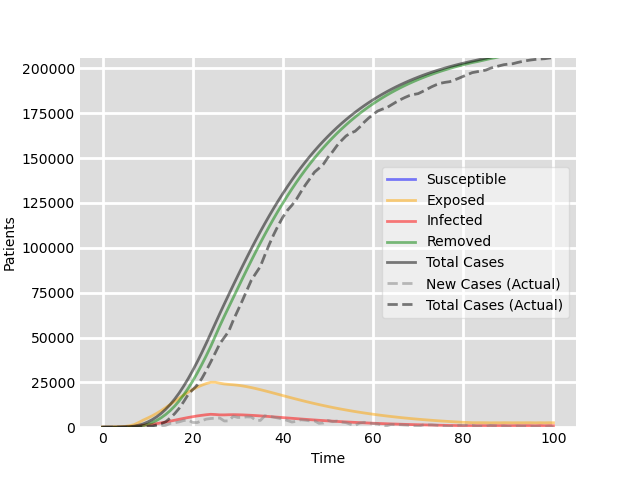
\includegraphics[width = 1.0\textwidth]{Scratch_Visuals/SEIR_Curve_NYC_2.png}
\end{figure}
\begin{figure}[htbp]
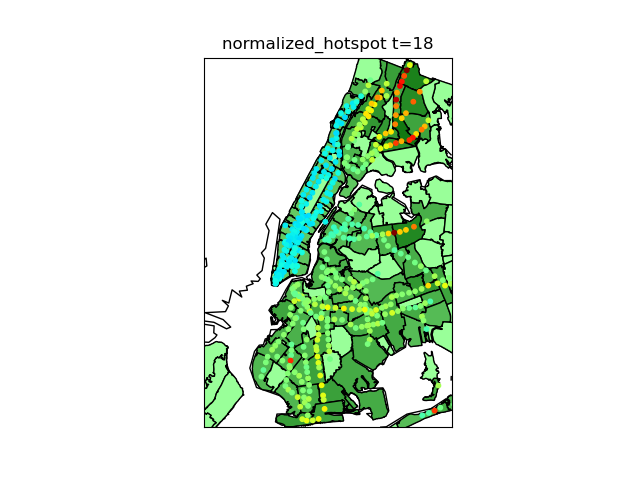
\includegraphics[width = 1.0\textwidth]{Scratch_Visuals/NYC_time018.png}
\end{figure}
\FloatBarrier
\textit{Writer's note: compare this to positive case coloring}
\section*{Conclusion}
\textbf{\textit{Writer's Note: All Models are Wrong, Some are Useful}}
\nocite{*}
\bibliography{bib_file}{}
\bibliographystyle{plain}

\end{document}
